\documentclass[11pt]{article}

    \usepackage[breakable]{tcolorbox}
    \usepackage{parskip} % Stop auto-indenting (to mimic markdown behaviour)
    
    \usepackage{iftex}
    \ifPDFTeX
    	\usepackage[T1]{fontenc}
    	\usepackage{mathpazo}
    \else
    	\usepackage{fontspec}
    \fi

    % Basic figure setup, for now with no caption control since it's done
    % automatically by Pandoc (which extracts ![](path) syntax from Markdown).
    \usepackage{graphicx}
    % Maintain compatibility with old templates. Remove in nbconvert 6.0
    \let\Oldincludegraphics\includegraphics
    % Ensure that by default, figures have no caption (until we provide a
    % proper Figure object with a Caption API and a way to capture that
    % in the conversion process - todo).
    \usepackage{caption}
    \DeclareCaptionFormat{nocaption}{}
    \captionsetup{format=nocaption,aboveskip=0pt,belowskip=0pt}

    \usepackage{float}
    \floatplacement{figure}{H} % forces figures to be placed at the correct location
    \usepackage{xcolor} % Allow colors to be defined
    \usepackage{enumerate} % Needed for markdown enumerations to work
    \usepackage{geometry} % Used to adjust the document margins
    \usepackage{amsmath} % Equations
    \usepackage{amssymb} % Equations
    \usepackage{textcomp} % defines textquotesingle
    % Hack from http://tex.stackexchange.com/a/47451/13684:
    \AtBeginDocument{%
        \def\PYZsq{\textquotesingle}% Upright quotes in Pygmentized code
    }
    \usepackage{upquote} % Upright quotes for verbatim code
    \usepackage{eurosym} % defines \euro
    \usepackage[mathletters]{ucs} % Extended unicode (utf-8) support
    \usepackage{fancyvrb} % verbatim replacement that allows latex
    \usepackage{grffile} % extends the file name processing of package graphics 
                         % to support a larger range
    \makeatletter % fix for old versions of grffile with XeLaTeX
    \@ifpackagelater{grffile}{2019/11/01}
    {
      % Do nothing on new versions
    }
    {
      \def\Gread@@xetex#1{%
        \IfFileExists{"\Gin@base".bb}%
        {\Gread@eps{\Gin@base.bb}}%
        {\Gread@@xetex@aux#1}%
      }
    }
    \makeatother
    \usepackage[Export]{adjustbox} % Used to constrain images to a maximum size
    \adjustboxset{max size={0.9\linewidth}{0.9\paperheight}}

    % The hyperref package gives us a pdf with properly built
    % internal navigation ('pdf bookmarks' for the table of contents,
    % internal cross-reference links, web links for URLs, etc.)
    \usepackage{hyperref}
    % The default LaTeX title has an obnoxious amount of whitespace. By default,
    % titling removes some of it. It also provides customization options.
    \usepackage{titling}
    \usepackage{longtable} % longtable support required by pandoc >1.10
    \usepackage{booktabs}  % table support for pandoc > 1.12.2
    \usepackage[inline]{enumitem} % IRkernel/repr support (it uses the enumerate* environment)
    \usepackage[normalem]{ulem} % ulem is needed to support strikethroughs (\sout)
                                % normalem makes italics be italics, not underlines
    \usepackage{mathrsfs}
    

    
    % Colors for the hyperref package
    \definecolor{urlcolor}{rgb}{0,.145,.698}
    \definecolor{linkcolor}{rgb}{.71,0.21,0.01}
    \definecolor{citecolor}{rgb}{.12,.54,.11}

    % ANSI colors
    \definecolor{ansi-black}{HTML}{3E424D}
    \definecolor{ansi-black-intense}{HTML}{282C36}
    \definecolor{ansi-red}{HTML}{E75C58}
    \definecolor{ansi-red-intense}{HTML}{B22B31}
    \definecolor{ansi-green}{HTML}{00A250}
    \definecolor{ansi-green-intense}{HTML}{007427}
    \definecolor{ansi-yellow}{HTML}{DDB62B}
    \definecolor{ansi-yellow-intense}{HTML}{B27D12}
    \definecolor{ansi-blue}{HTML}{208FFB}
    \definecolor{ansi-blue-intense}{HTML}{0065CA}
    \definecolor{ansi-magenta}{HTML}{D160C4}
    \definecolor{ansi-magenta-intense}{HTML}{A03196}
    \definecolor{ansi-cyan}{HTML}{60C6C8}
    \definecolor{ansi-cyan-intense}{HTML}{258F8F}
    \definecolor{ansi-white}{HTML}{C5C1B4}
    \definecolor{ansi-white-intense}{HTML}{A1A6B2}
    \definecolor{ansi-default-inverse-fg}{HTML}{FFFFFF}
    \definecolor{ansi-default-inverse-bg}{HTML}{000000}

    % common color for the border for error outputs.
    \definecolor{outerrorbackground}{HTML}{FFDFDF}

    % commands and environments needed by pandoc snippets
    % extracted from the output of `pandoc -s`
    \providecommand{\tightlist}{%
      \setlength{\itemsep}{0pt}\setlength{\parskip}{0pt}}
    \DefineVerbatimEnvironment{Highlighting}{Verbatim}{commandchars=\\\{\}}
    % Add ',fontsize=\small' for more characters per line
    \newenvironment{Shaded}{}{}
    \newcommand{\KeywordTok}[1]{\textcolor[rgb]{0.00,0.44,0.13}{\textbf{{#1}}}}
    \newcommand{\DataTypeTok}[1]{\textcolor[rgb]{0.56,0.13,0.00}{{#1}}}
    \newcommand{\DecValTok}[1]{\textcolor[rgb]{0.25,0.63,0.44}{{#1}}}
    \newcommand{\BaseNTok}[1]{\textcolor[rgb]{0.25,0.63,0.44}{{#1}}}
    \newcommand{\FloatTok}[1]{\textcolor[rgb]{0.25,0.63,0.44}{{#1}}}
    \newcommand{\CharTok}[1]{\textcolor[rgb]{0.25,0.44,0.63}{{#1}}}
    \newcommand{\StringTok}[1]{\textcolor[rgb]{0.25,0.44,0.63}{{#1}}}
    \newcommand{\CommentTok}[1]{\textcolor[rgb]{0.38,0.63,0.69}{\textit{{#1}}}}
    \newcommand{\OtherTok}[1]{\textcolor[rgb]{0.00,0.44,0.13}{{#1}}}
    \newcommand{\AlertTok}[1]{\textcolor[rgb]{1.00,0.00,0.00}{\textbf{{#1}}}}
    \newcommand{\FunctionTok}[1]{\textcolor[rgb]{0.02,0.16,0.49}{{#1}}}
    \newcommand{\RegionMarkerTok}[1]{{#1}}
    \newcommand{\ErrorTok}[1]{\textcolor[rgb]{1.00,0.00,0.00}{\textbf{{#1}}}}
    \newcommand{\NormalTok}[1]{{#1}}
    
    % Additional commands for more recent versions of Pandoc
    \newcommand{\ConstantTok}[1]{\textcolor[rgb]{0.53,0.00,0.00}{{#1}}}
    \newcommand{\SpecialCharTok}[1]{\textcolor[rgb]{0.25,0.44,0.63}{{#1}}}
    \newcommand{\VerbatimStringTok}[1]{\textcolor[rgb]{0.25,0.44,0.63}{{#1}}}
    \newcommand{\SpecialStringTok}[1]{\textcolor[rgb]{0.73,0.40,0.53}{{#1}}}
    \newcommand{\ImportTok}[1]{{#1}}
    \newcommand{\DocumentationTok}[1]{\textcolor[rgb]{0.73,0.13,0.13}{\textit{{#1}}}}
    \newcommand{\AnnotationTok}[1]{\textcolor[rgb]{0.38,0.63,0.69}{\textbf{\textit{{#1}}}}}
    \newcommand{\CommentVarTok}[1]{\textcolor[rgb]{0.38,0.63,0.69}{\textbf{\textit{{#1}}}}}
    \newcommand{\VariableTok}[1]{\textcolor[rgb]{0.10,0.09,0.49}{{#1}}}
    \newcommand{\ControlFlowTok}[1]{\textcolor[rgb]{0.00,0.44,0.13}{\textbf{{#1}}}}
    \newcommand{\OperatorTok}[1]{\textcolor[rgb]{0.40,0.40,0.40}{{#1}}}
    \newcommand{\BuiltInTok}[1]{{#1}}
    \newcommand{\ExtensionTok}[1]{{#1}}
    \newcommand{\PreprocessorTok}[1]{\textcolor[rgb]{0.74,0.48,0.00}{{#1}}}
    \newcommand{\AttributeTok}[1]{\textcolor[rgb]{0.49,0.56,0.16}{{#1}}}
    \newcommand{\InformationTok}[1]{\textcolor[rgb]{0.38,0.63,0.69}{\textbf{\textit{{#1}}}}}
    \newcommand{\WarningTok}[1]{\textcolor[rgb]{0.38,0.63,0.69}{\textbf{\textit{{#1}}}}}
    
    
    % Define a nice break command that doesn't care if a line doesn't already
    % exist.
    \def\br{\hspace*{\fill} \\* }
    % Math Jax compatibility definitions
    \def\gt{>}
    \def\lt{<}
    \let\Oldtex\TeX
    \let\Oldlatex\LaTeX
    \renewcommand{\TeX}{\textrm{\Oldtex}}
    \renewcommand{\LaTeX}{\textrm{\Oldlatex}}
    % Document parameters
    % Document title
    %\title{Collaborative Spectrum Sharing Lab}

   
    
    
    
    
% Pygments definitions
\makeatletter
\def\PY@reset{\let\PY@it=\relax \let\PY@bf=\relax%
    \let\PY@ul=\relax \let\PY@tc=\relax%
    \let\PY@bc=\relax \let\PY@ff=\relax}
\def\PY@tok#1{\csname PY@tok@#1\endcsname}
\def\PY@toks#1+{\ifx\relax#1\empty\else%
    \PY@tok{#1}\expandafter\PY@toks\fi}
\def\PY@do#1{\PY@bc{\PY@tc{\PY@ul{%
    \PY@it{\PY@bf{\PY@ff{#1}}}}}}}
\def\PY#1#2{\PY@reset\PY@toks#1+\relax+\PY@do{#2}}

\@namedef{PY@tok@w}{\def\PY@tc##1{\textcolor[rgb]{0.73,0.73,0.73}{##1}}}
\@namedef{PY@tok@c}{\let\PY@it=\textit\def\PY@tc##1{\textcolor[rgb]{0.25,0.50,0.50}{##1}}}
\@namedef{PY@tok@cp}{\def\PY@tc##1{\textcolor[rgb]{0.74,0.48,0.00}{##1}}}
\@namedef{PY@tok@k}{\let\PY@bf=\textbf\def\PY@tc##1{\textcolor[rgb]{0.00,0.50,0.00}{##1}}}
\@namedef{PY@tok@kp}{\def\PY@tc##1{\textcolor[rgb]{0.00,0.50,0.00}{##1}}}
\@namedef{PY@tok@kt}{\def\PY@tc##1{\textcolor[rgb]{0.69,0.00,0.25}{##1}}}
\@namedef{PY@tok@o}{\def\PY@tc##1{\textcolor[rgb]{0.40,0.40,0.40}{##1}}}
\@namedef{PY@tok@ow}{\let\PY@bf=\textbf\def\PY@tc##1{\textcolor[rgb]{0.67,0.13,1.00}{##1}}}
\@namedef{PY@tok@nb}{\def\PY@tc##1{\textcolor[rgb]{0.00,0.50,0.00}{##1}}}
\@namedef{PY@tok@nf}{\def\PY@tc##1{\textcolor[rgb]{0.00,0.00,1.00}{##1}}}
\@namedef{PY@tok@nc}{\let\PY@bf=\textbf\def\PY@tc##1{\textcolor[rgb]{0.00,0.00,1.00}{##1}}}
\@namedef{PY@tok@nn}{\let\PY@bf=\textbf\def\PY@tc##1{\textcolor[rgb]{0.00,0.00,1.00}{##1}}}
\@namedef{PY@tok@ne}{\let\PY@bf=\textbf\def\PY@tc##1{\textcolor[rgb]{0.82,0.25,0.23}{##1}}}
\@namedef{PY@tok@nv}{\def\PY@tc##1{\textcolor[rgb]{0.10,0.09,0.49}{##1}}}
\@namedef{PY@tok@no}{\def\PY@tc##1{\textcolor[rgb]{0.53,0.00,0.00}{##1}}}
\@namedef{PY@tok@nl}{\def\PY@tc##1{\textcolor[rgb]{0.63,0.63,0.00}{##1}}}
\@namedef{PY@tok@ni}{\let\PY@bf=\textbf\def\PY@tc##1{\textcolor[rgb]{0.60,0.60,0.60}{##1}}}
\@namedef{PY@tok@na}{\def\PY@tc##1{\textcolor[rgb]{0.49,0.56,0.16}{##1}}}
\@namedef{PY@tok@nt}{\let\PY@bf=\textbf\def\PY@tc##1{\textcolor[rgb]{0.00,0.50,0.00}{##1}}}
\@namedef{PY@tok@nd}{\def\PY@tc##1{\textcolor[rgb]{0.67,0.13,1.00}{##1}}}
\@namedef{PY@tok@s}{\def\PY@tc##1{\textcolor[rgb]{0.73,0.13,0.13}{##1}}}
\@namedef{PY@tok@sd}{\let\PY@it=\textit\def\PY@tc##1{\textcolor[rgb]{0.73,0.13,0.13}{##1}}}
\@namedef{PY@tok@si}{\let\PY@bf=\textbf\def\PY@tc##1{\textcolor[rgb]{0.73,0.40,0.53}{##1}}}
\@namedef{PY@tok@se}{\let\PY@bf=\textbf\def\PY@tc##1{\textcolor[rgb]{0.73,0.40,0.13}{##1}}}
\@namedef{PY@tok@sr}{\def\PY@tc##1{\textcolor[rgb]{0.73,0.40,0.53}{##1}}}
\@namedef{PY@tok@ss}{\def\PY@tc##1{\textcolor[rgb]{0.10,0.09,0.49}{##1}}}
\@namedef{PY@tok@sx}{\def\PY@tc##1{\textcolor[rgb]{0.00,0.50,0.00}{##1}}}
\@namedef{PY@tok@m}{\def\PY@tc##1{\textcolor[rgb]{0.40,0.40,0.40}{##1}}}
\@namedef{PY@tok@gh}{\let\PY@bf=\textbf\def\PY@tc##1{\textcolor[rgb]{0.00,0.00,0.50}{##1}}}
\@namedef{PY@tok@gu}{\let\PY@bf=\textbf\def\PY@tc##1{\textcolor[rgb]{0.50,0.00,0.50}{##1}}}
\@namedef{PY@tok@gd}{\def\PY@tc##1{\textcolor[rgb]{0.63,0.00,0.00}{##1}}}
\@namedef{PY@tok@gi}{\def\PY@tc##1{\textcolor[rgb]{0.00,0.63,0.00}{##1}}}
\@namedef{PY@tok@gr}{\def\PY@tc##1{\textcolor[rgb]{1.00,0.00,0.00}{##1}}}
\@namedef{PY@tok@ge}{\let\PY@it=\textit}
\@namedef{PY@tok@gs}{\let\PY@bf=\textbf}
\@namedef{PY@tok@gp}{\let\PY@bf=\textbf\def\PY@tc##1{\textcolor[rgb]{0.00,0.00,0.50}{##1}}}
\@namedef{PY@tok@go}{\def\PY@tc##1{\textcolor[rgb]{0.53,0.53,0.53}{##1}}}
\@namedef{PY@tok@gt}{\def\PY@tc##1{\textcolor[rgb]{0.00,0.27,0.87}{##1}}}
\@namedef{PY@tok@err}{\def\PY@bc##1{{\setlength{\fboxsep}{\string -\fboxrule}\fcolorbox[rgb]{1.00,0.00,0.00}{1,1,1}{\strut ##1}}}}
\@namedef{PY@tok@kc}{\let\PY@bf=\textbf\def\PY@tc##1{\textcolor[rgb]{0.00,0.50,0.00}{##1}}}
\@namedef{PY@tok@kd}{\let\PY@bf=\textbf\def\PY@tc##1{\textcolor[rgb]{0.00,0.50,0.00}{##1}}}
\@namedef{PY@tok@kn}{\let\PY@bf=\textbf\def\PY@tc##1{\textcolor[rgb]{0.00,0.50,0.00}{##1}}}
\@namedef{PY@tok@kr}{\let\PY@bf=\textbf\def\PY@tc##1{\textcolor[rgb]{0.00,0.50,0.00}{##1}}}
\@namedef{PY@tok@bp}{\def\PY@tc##1{\textcolor[rgb]{0.00,0.50,0.00}{##1}}}
\@namedef{PY@tok@fm}{\def\PY@tc##1{\textcolor[rgb]{0.00,0.00,1.00}{##1}}}
\@namedef{PY@tok@vc}{\def\PY@tc##1{\textcolor[rgb]{0.10,0.09,0.49}{##1}}}
\@namedef{PY@tok@vg}{\def\PY@tc##1{\textcolor[rgb]{0.10,0.09,0.49}{##1}}}
\@namedef{PY@tok@vi}{\def\PY@tc##1{\textcolor[rgb]{0.10,0.09,0.49}{##1}}}
\@namedef{PY@tok@vm}{\def\PY@tc##1{\textcolor[rgb]{0.10,0.09,0.49}{##1}}}
\@namedef{PY@tok@sa}{\def\PY@tc##1{\textcolor[rgb]{0.73,0.13,0.13}{##1}}}
\@namedef{PY@tok@sb}{\def\PY@tc##1{\textcolor[rgb]{0.73,0.13,0.13}{##1}}}
\@namedef{PY@tok@sc}{\def\PY@tc##1{\textcolor[rgb]{0.73,0.13,0.13}{##1}}}
\@namedef{PY@tok@dl}{\def\PY@tc##1{\textcolor[rgb]{0.73,0.13,0.13}{##1}}}
\@namedef{PY@tok@s2}{\def\PY@tc##1{\textcolor[rgb]{0.73,0.13,0.13}{##1}}}
\@namedef{PY@tok@sh}{\def\PY@tc##1{\textcolor[rgb]{0.73,0.13,0.13}{##1}}}
\@namedef{PY@tok@s1}{\def\PY@tc##1{\textcolor[rgb]{0.73,0.13,0.13}{##1}}}
\@namedef{PY@tok@mb}{\def\PY@tc##1{\textcolor[rgb]{0.40,0.40,0.40}{##1}}}
\@namedef{PY@tok@mf}{\def\PY@tc##1{\textcolor[rgb]{0.40,0.40,0.40}{##1}}}
\@namedef{PY@tok@mh}{\def\PY@tc##1{\textcolor[rgb]{0.40,0.40,0.40}{##1}}}
\@namedef{PY@tok@mi}{\def\PY@tc##1{\textcolor[rgb]{0.40,0.40,0.40}{##1}}}
\@namedef{PY@tok@il}{\def\PY@tc##1{\textcolor[rgb]{0.40,0.40,0.40}{##1}}}
\@namedef{PY@tok@mo}{\def\PY@tc##1{\textcolor[rgb]{0.40,0.40,0.40}{##1}}}
\@namedef{PY@tok@ch}{\let\PY@it=\textit\def\PY@tc##1{\textcolor[rgb]{0.25,0.50,0.50}{##1}}}
\@namedef{PY@tok@cm}{\let\PY@it=\textit\def\PY@tc##1{\textcolor[rgb]{0.25,0.50,0.50}{##1}}}
\@namedef{PY@tok@cpf}{\let\PY@it=\textit\def\PY@tc##1{\textcolor[rgb]{0.25,0.50,0.50}{##1}}}
\@namedef{PY@tok@c1}{\let\PY@it=\textit\def\PY@tc##1{\textcolor[rgb]{0.25,0.50,0.50}{##1}}}
\@namedef{PY@tok@cs}{\let\PY@it=\textit\def\PY@tc##1{\textcolor[rgb]{0.25,0.50,0.50}{##1}}}

\def\PYZbs{\char`\\}
\def\PYZus{\char`\_}
\def\PYZob{\char`\{}
\def\PYZcb{\char`\}}
\def\PYZca{\char`\^}
\def\PYZam{\char`\&}
\def\PYZlt{\char`\<}
\def\PYZgt{\char`\>}
\def\PYZsh{\char`\#}
\def\PYZpc{\char`\%}
\def\PYZdl{\char`\$}
\def\PYZhy{\char`\-}
\def\PYZsq{\char`\'}
\def\PYZdq{\char`\"}
\def\PYZti{\char`\~}
% for compatibility with earlier versions
\def\PYZat{@}
\def\PYZlb{[}
\def\PYZrb{]}
\makeatother


    % For linebreaks inside Verbatim environment from package fancyvrb. 
    \makeatletter
        \newbox\Wrappedcontinuationbox 
        \newbox\Wrappedvisiblespacebox 
        \newcommand*\Wrappedvisiblespace {\textcolor{red}{\textvisiblespace}} 
        \newcommand*\Wrappedcontinuationsymbol {\textcolor{red}{\llap{\tiny$\m@th\hookrightarrow$}}} 
        \newcommand*\Wrappedcontinuationindent {3ex } 
        \newcommand*\Wrappedafterbreak {\kern\Wrappedcontinuationindent\copy\Wrappedcontinuationbox} 
        % Take advantage of the already applied Pygments mark-up to insert 
        % potential linebreaks for TeX processing. 
        %        {, <, #, %, $, ' and ": go to next line. 
        %        _, }, ^, &, >, - and ~: stay at end of broken line. 
        % Use of \textquotesingle for straight quote. 
        \newcommand*\Wrappedbreaksatspecials {% 
            \def\PYGZus{\discretionary{\char`\_}{\Wrappedafterbreak}{\char`\_}}% 
            \def\PYGZob{\discretionary{}{\Wrappedafterbreak\char`\{}{\char`\{}}% 
            \def\PYGZcb{\discretionary{\char`\}}{\Wrappedafterbreak}{\char`\}}}% 
            \def\PYGZca{\discretionary{\char`\^}{\Wrappedafterbreak}{\char`\^}}% 
            \def\PYGZam{\discretionary{\char`\&}{\Wrappedafterbreak}{\char`\&}}% 
            \def\PYGZlt{\discretionary{}{\Wrappedafterbreak\char`\<}{\char`\<}}% 
            \def\PYGZgt{\discretionary{\char`\>}{\Wrappedafterbreak}{\char`\>}}% 
            \def\PYGZsh{\discretionary{}{\Wrappedafterbreak\char`\#}{\char`\#}}% 
            \def\PYGZpc{\discretionary{}{\Wrappedafterbreak\char`\%}{\char`\%}}% 
            \def\PYGZdl{\discretionary{}{\Wrappedafterbreak\char`\$}{\char`\$}}% 
            \def\PYGZhy{\discretionary{\char`\-}{\Wrappedafterbreak}{\char`\-}}% 
            \def\PYGZsq{\discretionary{}{\Wrappedafterbreak\textquotesingle}{\textquotesingle}}% 
            \def\PYGZdq{\discretionary{}{\Wrappedafterbreak\char`\"}{\char`\"}}% 
            \def\PYGZti{\discretionary{\char`\~}{\Wrappedafterbreak}{\char`\~}}% 
        } 
        % Some characters . , ; ? ! / are not pygmentized. 
        % This macro makes them "active" and they will insert potential linebreaks 
        \newcommand*\Wrappedbreaksatpunct {% 
            \lccode`\~`\.\lowercase{\def~}{\discretionary{\hbox{\char`\.}}{\Wrappedafterbreak}{\hbox{\char`\.}}}% 
            \lccode`\~`\,\lowercase{\def~}{\discretionary{\hbox{\char`\,}}{\Wrappedafterbreak}{\hbox{\char`\,}}}% 
            \lccode`\~`\;\lowercase{\def~}{\discretionary{\hbox{\char`\;}}{\Wrappedafterbreak}{\hbox{\char`\;}}}% 
            \lccode`\~`\:\lowercase{\def~}{\discretionary{\hbox{\char`\:}}{\Wrappedafterbreak}{\hbox{\char`\:}}}% 
            \lccode`\~`\?\lowercase{\def~}{\discretionary{\hbox{\char`\?}}{\Wrappedafterbreak}{\hbox{\char`\?}}}% 
            \lccode`\~`\!\lowercase{\def~}{\discretionary{\hbox{\char`\!}}{\Wrappedafterbreak}{\hbox{\char`\!}}}% 
            \lccode`\~`\/\lowercase{\def~}{\discretionary{\hbox{\char`\/}}{\Wrappedafterbreak}{\hbox{\char`\/}}}% 
            \catcode`\.\active
            \catcode`\,\active 
            \catcode`\;\active
            \catcode`\:\active
            \catcode`\?\active
            \catcode`\!\active
            \catcode`\/\active 
            \lccode`\~`\~ 	
        }
    \makeatother

    \let\OriginalVerbatim=\Verbatim
    \makeatletter
    \renewcommand{\Verbatim}[1][1]{%
        %\parskip\z@skip
        \sbox\Wrappedcontinuationbox {\Wrappedcontinuationsymbol}%
        \sbox\Wrappedvisiblespacebox {\FV@SetupFont\Wrappedvisiblespace}%
        \def\FancyVerbFormatLine ##1{\hsize\linewidth
            \vtop{\raggedright\hyphenpenalty\z@\exhyphenpenalty\z@
                \doublehyphendemerits\z@\finalhyphendemerits\z@
                \strut ##1\strut}%
        }%
        % If the linebreak is at a space, the latter will be displayed as visible
        % space at end of first line, and a continuation symbol starts next line.
        % Stretch/shrink are however usually zero for typewriter font.
        \def\FV@Space {%
            \nobreak\hskip\z@ plus\fontdimen3\font minus\fontdimen4\font
            \discretionary{\copy\Wrappedvisiblespacebox}{\Wrappedafterbreak}
            {\kern\fontdimen2\font}%
        }%
        
        % Allow breaks at special characters using \PYG... macros.
        \Wrappedbreaksatspecials
        % Breaks at punctuation characters . , ; ? ! and / need catcode=\active 	
        \OriginalVerbatim[#1,codes*=\Wrappedbreaksatpunct]%
    }
    \makeatother

    % Exact colors from NB
    \definecolor{incolor}{HTML}{303F9F}
    \definecolor{outcolor}{HTML}{D84315}
    \definecolor{cellborder}{HTML}{CFCFCF}
    \definecolor{cellbackground}{HTML}{F7F7F7}
    
    % prompt
    \makeatletter
    \newcommand{\boxspacing}{\kern\kvtcb@left@rule\kern\kvtcb@boxsep}
    \makeatother
    \newcommand{\prompt}[4]{
        {\ttfamily\llap{{\color{#2}[#3]:\hspace{3pt}#4}}\vspace{-\baselineskip}}
    }
    

    
    % Prevent overflowing lines due to hard-to-break entities
    \sloppy 
    % Setup hyperref package
    \hypersetup{
      breaklinks=true,  % so long urls are correctly broken across lines
      colorlinks=true,
      urlcolor=urlcolor,
      linkcolor=linkcolor,
      citecolor=citecolor,
      }
    % Slightly bigger margins than the latex defaults
    
    \geometry{verbose,tmargin=1in,bmargin=1in,lmargin=1in,rmargin=1in}
    
    

\begin{document}
    
    %\maketitle
    \begin{center}
{\Huge 
    Collaborative Spectrum Sharing Lab}
\end{center}
 
    

    
    \hypertarget{lab-handout}{%
\section*{Lab Handout}\label{lab-handout}}

Your Name: \underline{\hspace*{3 in}}


\hypertarget{part-1-getting-to-know-audio-frequencies-visualizing-sounds-of-tuning-forks}{%
\section*{Part 1: Getting to Know Audio Frequencies: Visualizing Sounds
of Tuning
Forks}\label{part-1-getting-to-know-audio-frequencies-visualizing-sounds-of-tuning-forks}}

\hypertarget{visualizing-the-data-time-domain}{%
\subsubsection*{Visualizing the Data (Time
Domain)}\label{visualizing-the-data-time-domain}}

\textbf{Question 1.1: Does anyone know what this type of signal or
function is called?}

\hypertarget{comparing-audio-signals-for-tuning-forks-with-different-tunings}{%
\subsubsection*{Comparing Audio Signals for Tuning Forks with Different
Tunings}\label{comparing-audio-signals-for-tuning-forks-with-different-tunings}}

\textbf{QUESTION 1.2: How would you describe the relation between the
``Beethoven A'' and ``UF E'' waves?}

\begin{longtable}[]{@{}l@{}}
\toprule
 \\
\midrule
\endhead
 \\
 \\
 \\
\bottomrule
\end{longtable}

\textbf{QUESTION 1.3: What is different between the plots shown of the
``Beethoven A'' and ``UF E'' waves?}

\begin{longtable}[]{@{}l@{}}
\toprule
 \\
\midrule
\endhead
 \\
 \\
 \\
\bottomrule
\end{longtable}

\textbf{Question 1.4: Ignoring the small fluctuations in the recording,
what do you notice that is different about the two plots of individual
cycles of the ``Beethoven A'' and ``UF E'' waves?}

\begin{longtable}[]{@{}l@{}}
\toprule
 \\
\midrule
\endhead
 \\
 \\
 \\
\bottomrule
\end{longtable}

\newpage
\hypertarget{making-waves}{%
\subsubsection*{Making Waves}\label{making-waves}}

\textbf{Question 1.5: Circle the appropriate relation in each sentence:}
* Beethoven's tuning fork sounded \textbf{higher / lower} than the UF E
tuning fork.

\begin{longtable}[]{@{}l@{}}
\toprule
 \\
\midrule
\endhead
 \\
\bottomrule
\end{longtable}

\begin{itemize}
\tightlist
\item
  For a fixed observation time of 0.01 s, we observed that Beethoven's
  tuning had \textbf{more / fewer} cycles than the UF E tuning fork.
\end{itemize}

\begin{longtable}[]{@{}l@{}}
\toprule
 \\
\midrule
\endhead
 \\
\bottomrule
\end{longtable}

\begin{itemize}
\tightlist
\item
  One cycle of the Beethoven's tuning fork took \textbf{more / less}
  time than one cycle of the UF E tuning fork.
\end{itemize}

\begin{longtable}[]{@{}l@{}}
\toprule
 \\
\midrule
\endhead
 \\
\bottomrule
\end{longtable}

\textbf{Question 1.6: How does the \texttt{cycle\_rate} parameter effect
the pitch of the audio signal?}

\begin{longtable}[]{@{}l@{}}
\toprule
 \\
\midrule
\endhead
 \\
 \\
 \\
\bottomrule
\end{longtable}

    \begin{center}\rule{\linewidth}{0.5pt}\end{center}

\hypertarget{part-2-getting-to-know-audio-frequencies-defining-frequency-and-visualizing-frequencies-of-signals}{%
\section*{Part 2: Getting to Know Audio Frequencies: Defining Frequency
and Visualizing Frequencies of
Signals}\label{part-2-getting-to-know-audio-frequencies-defining-frequency-and-visualizing-frequencies-of-signals}}

\hypertarget{frequency}{%
\subsubsection*{Frequency}\label{frequency}}

\textbf{Question 2.1: What do you think the word \emph{frequency} means?
In what contexts have you heard that term?}

\begin{longtable}[]{@{}l@{}}
\toprule
 \\
\midrule
\endhead
 \\
 \\
 \\
\bottomrule
\end{longtable}

\hypertarget{what-frequencies-can-you-hear}{%
\subsubsection*{What frequencies can you
hear?}\label{what-frequencies-can-you-hear}}

\textbf{Activity 2.2:} 1. Write down the lowest frequency that you can
hear. 1. Write down the lowest frequency that still sounds like a
musical note to you.

\begin{longtable}[]{@{}l@{}}
\toprule
 \\
\midrule
\endhead
 \\
 \\
 \\
\bottomrule
\end{longtable}

\textbf{Activity 2.3: Write down the highest frequency that you can
hear. Compare with the other students in the lab. Compare with the lab
instructor.}

\begin{longtable}[]{@{}l@{}}
\toprule
 \\
\midrule
\endhead
 \\
 \\
 \\
\bottomrule
\end{longtable}

\hypertarget{richer-audio-guitar}{%
\subsubsection*{Richer Audio: Guitar}\label{richer-audio-guitar}}

\textbf{Question 2.4: What do you observe? How is this similar to, and
different from, the tuning fork signals?}

\begin{longtable}[]{@{}l@{}}
\toprule
 \\
\midrule
\endhead
 \\
 \\
 \\
\bottomrule
\end{longtable}

\textbf{Question 2.5: Recall that the E note is at about 330 Hz. How do
the other components in this plot relate to that frequency?}

\begin{longtable}[]{@{}l@{}}
\toprule
 \\
\midrule
\endhead
 \\
 \\
 \\
\bottomrule
\end{longtable}

\textbf{Activity 2.6: Write down the number of harmonics you feel are
needed for the resulting signal to like the original guitar.}

\begin{longtable}[]{@{}l@{}}
\toprule
 \\
\midrule
\endhead
 \\
 \\
 \\
\bottomrule
\end{longtable}

\hypertarget{analyzing-voice-data}{%
\subsubsection*{Analyzing Voice Data}\label{analyzing-voice-data}}

\textbf{Activity 2.7: How many harmonics are needed before this sounds
like a voice?}

\begin{longtable}[]{@{}l@{}}
\toprule
 \\
\midrule
\endhead
 \\
 \\
 \\
\bottomrule
\end{longtable}

\textbf{Activity 2.8 (Optional, requires recording): Go back and record
human speech and repeat all the voice data analysis. How is the time
signal different than for singing a note? How is the frequency signal
different than for singing a note?}

\begin{longtable}[]{@{}l@{}}
\toprule
 \\
\midrule
\endhead
 \\
 \\
 \\
\bottomrule
\end{longtable}

    \begin{center}\rule{\linewidth}{0.5pt}\end{center}

\hypertarget{part-3-frequency-multiplexing-transmitting-multiple-voice-signals}{%
\section*{Part 3: Frequency Multiplexing: Transmitting Multiple Voice
Signals}\label{part-3-frequency-multiplexing-transmitting-multiple-voice-signals}}

\hypertarget{frequency-multiplexing-part-1-low-pass-filtering}{%
\subsubsection*{Frequency Multiplexing: Part 1 -- Low Pass
Filtering}\label{frequency-multiplexing-part-1-low-pass-filtering}}

\textbf{Question 3.1: How do the filtered signals sound in comparison to
the original signals?}

\begin{longtable}[]{@{}l@{}}
\toprule
 \\
\midrule
\endhead
 \\
 \\
 \\
\bottomrule
\end{longtable}

\hypertarget{frequency-multiplexing-part-2-frequency-shifting-and-combining}{%
\subsubsection*{Frequency Multiplexing: Part 2 -- Frequency Shifting and
Combining}\label{frequency-multiplexing-part-2-frequency-shifting-and-combining}}

\textbf{Question 3.2: Describe how the frequency-shifted signal sounds
compared to the original signal.}

\begin{longtable}[]{@{}l@{}}
\toprule
 \\
\midrule
\endhead
 \\
 \\
 \\
\bottomrule
\end{longtable}

\newpage
\textbf{Question 3.3: How does the plot of the frequency-shifted signal
compare to the plot of the original signal?}

\begin{longtable}[]{@{}l@{}}
\toprule
 \\
\midrule
\endhead
 \\
 \\
 \\
\bottomrule
\end{longtable}

\textbf{Activity 3.4: Listen to the combined signal. Can you hear the
different messages? Propose an explanation for what you have heard.}

\begin{longtable}[]{@{}l@{}}
\toprule
 \\
\midrule
\endhead
 \\
 \\
 \\
\bottomrule
\end{longtable}

\hypertarget{frequency-demultiplexing}{%
\subsection*{Frequency Demultiplexing}\label{frequency-demultiplexing}}

\textbf{Questions 3.5: Do you hear any differences between the
demultiplexed signals and the filtered signals? Why do you think you
did/did not?}

\begin{longtable}[]{@{}l@{}}
\toprule
 \\
\midrule
\endhead
 \\
 \\
 \\
\bottomrule
\end{longtable}

\hypertarget{review}{%
\subsection*{Review}\label{review}}

\begin{itemize}
\tightlist
\item
  Frequency-division multiplexing is a way to put multiple signals on
  different, non-overlapping frequency bands
\item
  The FFT and IFFT are techniques to transform signals into frequency
  representations, where filtering out frequencies or shifting
  frequencies are easily done
\item
  Demultiplexing is the process of recovering the individual signals
  that have been multiplexed together.
\end{itemize}

    \begin{center}\rule{\linewidth}{0.5pt}\end{center}
    \newpage

\hypertarget{part-4-scanning-the-radio-spectrum}{%
\section*{Part 4: Scanning the Radio
Spectrum}\label{part-4-scanning-the-radio-spectrum}}

\hypertarget{fm-radio}{%
\subsubsection*{FM Radio}\label{fm-radio}}

\textbf{Activity 4.1 Identify at least two other strong radio signals.
Find out the four-letter ID and type of radio station.}

\begin{longtable}[]{@{}l@{}}
\toprule
 \\
\midrule
\endhead
 \\
 \\
 \\
\bottomrule
\end{longtable}

\hypertarget{cellular-band}{%
\subsubsection*{Cellular Band}\label{cellular-band}}

\textbf{Activity 4.2 Estimate the center frequency and the bandwidth
(the amount of frequency spanned by the signal) for several of the
signals observed.}

\begin{longtable}[]{@{}l@{}}
\toprule
 \\
\midrule
\endhead
 \\
 \\
 \\
\bottomrule
\end{longtable}

    \begin{center}\rule{\linewidth}{0.5pt}\end{center}

    \hypertarget{part-5.-digital-modulation}{%
\section*{Part 5. Digital
Modulation}\label{part-5.-digital-modulation}}

    \hypertarget{on-off-keying}{%
\subsubsection*{On-Off Keying}\label{on-off-keying}}

\textbf{Question 5.1 What problems might there be with using On-Off
Keying to send information? How might you avoid those problems?}

\begin{longtable}[]{@{}l@{}}
\toprule
 \\
\midrule
\endhead
 \\
 \\
 \\
\bottomrule
\end{longtable}

    \textbf{Activity 5.2: Adjust the \texttt{noise\_variance} parameter
above to see how it affects the performance of this system.}

\begin{itemize}
\tightlist
\item
  How high can \texttt{noise\_variance} be before you start to see a
  large number of errors.
\end{itemize}

\begin{longtable}[]{@{}l@{}}
\toprule
 \\
\midrule
\endhead
 \\
 \\
 \\
\bottomrule
\end{longtable}

\begin{itemize}
\tightlist
\item
  Is one type of error more prevalent than another? Why do you think
  that is the case?
\end{itemize}

\begin{longtable}[]{@{}l@{}}
\toprule
 \\
\midrule
\endhead
 \\
 \\
 \\
\bottomrule
\end{longtable}

\begin{itemize}
\tightlist
\item
  Can you think of any way to improve the performance of this detector
  when the noise is large?
\end{itemize}

\begin{longtable}[]{@{}l@{}}
\toprule
 \\
\midrule
\endhead
 \\
 \\
 \\
\bottomrule
\end{longtable}

\begin{itemize}
\tightlist
\item
  Try to modify the code to improve the performance when the noise is
  large. Were you successful? If so, what did you do and why?
\end{itemize}

\begin{longtable}[]{@{}l@{}}
\toprule
 \\
\midrule
\endhead
 \\
 \\
 \\
\bottomrule
\end{longtable}

\textbf{Activity 5.3:} For the where you listen to a modulated message
that consists of a 1 followed by 5 random bits, write down your record
as:

\# correct / \# tries

(like 3/5)

\begin{longtable}[]{@{}l@{}}
\toprule
 \\
\midrule
\endhead
 \\
 \\
 \\
\bottomrule
\end{longtable}

    \hypertarget{on-off-keying-morse-code}{%
\subsubsection*{On-Off Keying: Morse
Code}\label{on-off-keying-morse-code}}

\begin{figure}
\centering
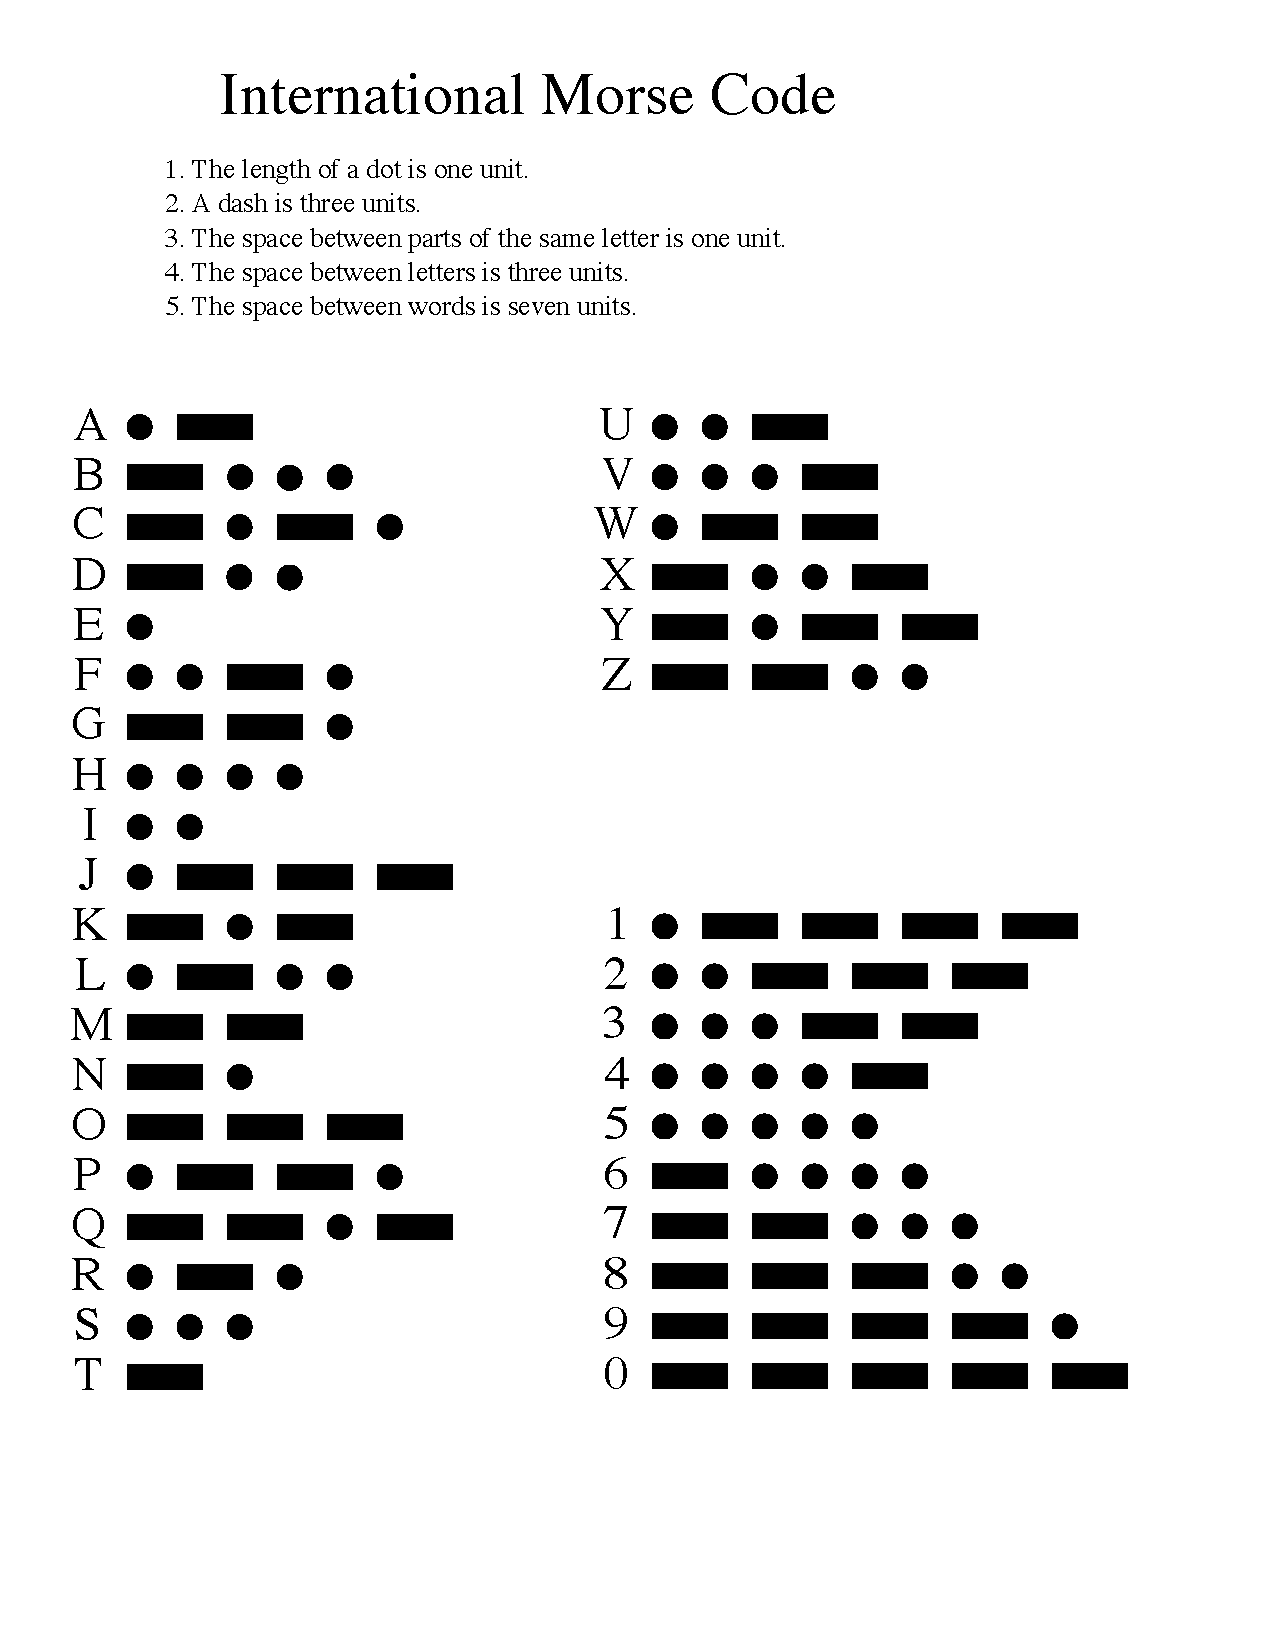
\includegraphics{plots/morse.pdf}
\caption{From Rhey T. Snodgrass \& Victor F. Camp, 1922}
\end{figure}

\newpage
    \textbf{Activity 5.4:} The Morse Code activity uses a parameter called
\texttt{dit\_duration}. Try setting \texttt{dit\_duration} to a smaller
value, such as 0.05. Write down the smallest value of
\texttt{dit\_durration} at which you can still reliably decode the
message.

\begin{longtable}[]{@{}l@{}}
\toprule
 \\
\midrule
\endhead
 \\
 \\
 \\
\bottomrule
\end{longtable}

    \hypertarget{review}{%
\subsubsection*{Review}\label{review}}

\begin{itemize}
\tightlist
\item
  \emph{Modulation} is the process by information is encoded for
  transmission on a channel.
\item
  In \emph{on-off keying}, an information stream is conveyed by turning
  a carrier on and off.
\item
  \emph{Demodulation} is the process of taking a modulated signal and
  recovering the information.
\item
  \emph{Morse Code} is a way to efficiently modulate English letters and
  numbers as a sequence of tones of varying lengths.
\end{itemize}

\begin{center}\rule{\linewidth}{0.5pt}\end{center}

    \hypertarget{part-6.-spectrum-sharing}{%
\section*{Part 6. Spectrum Sharing}\label{part-6.-spectrum-sharing}}

    \textbf{Activity 6.1: Volume Normalization}

Write down your team number:

\begin{longtable}[]{@{}l@{}}
\toprule
 \\
\midrule
\endhead
 \\
 \\
 \\
\bottomrule
\end{longtable}

\hypertarget{spectrum-sharing-with-fixed-assignments-1}{%
\subsubsection*{Spectrum Sharing with Fixed Assignments
1}\label{spectrum-sharing-with-fixed-assignments-1}}

\textbf{Activity 6.2: Simultaneous Transmission Fixed Frequencies}

If you team is transmitting during the following tests, write down the
message that was guessed by the human receivers and the actual message
transmitted.** 1. Teams 1 and 3 run the block below simultaneously.

\begin{longtable}[]{@{}l@{}}
\toprule
 \\
\midrule
\endhead
 \\
 \\
 \\
\bottomrule
\end{longtable}

\begin{enumerate}
\def\labelenumi{\arabic{enumi}.}
\setcounter{enumi}{1}
\tightlist
\item
  Teams 2 and 4 run the block below simultaneously.
\end{enumerate}

\begin{longtable}[]{@{}l@{}}
\toprule
 \\
\midrule
\endhead
 \\
 \\
 \\
\bottomrule
\end{longtable}

\begin{enumerate}
\def\labelenumi{\arabic{enumi}.}
\setcounter{enumi}{2}
\tightlist
\item
  Teams 1, 2, and 4 run the block below simultaneously.
\end{enumerate}

\begin{longtable}[]{@{}l@{}}
\toprule
 \\
\midrule
\endhead
 \\
 \\
 \\
\bottomrule
\end{longtable}

\begin{enumerate}
\def\labelenumi{\arabic{enumi}.}
\setcounter{enumi}{3}
\tightlist
\item
  Teams 1, 3, and 4 run the block below simultaneously.
\end{enumerate}

\begin{longtable}[]{@{}l@{}}
\toprule
 \\
\midrule
\endhead
 \\
 \\
 \\
\bottomrule
\end{longtable}

\begin{enumerate}
\def\labelenumi{\arabic{enumi}.}
\setcounter{enumi}{4}
\tightlist
\item
  All teams run the block below simultaneously.
\end{enumerate}

\begin{longtable}[]{@{}l@{}}
\toprule
 \\
\midrule
\endhead
 \\
 \\
 \\
\bottomrule
\end{longtable}

    \hypertarget{spectrum-sharing-with-fixed-assignments-2}{%
\subsubsection*{Spectrum Sharing with Fixed Assignments
2}\label{spectrum-sharing-with-fixed-assignments-2}}

\textbf{Activity 6.3: Using a Tuned Receiver}

\emph{Sketch what the output of the tuned receiver looks like.}

\begin{longtable}[]{@{}l@{}}
\toprule
 \\
\midrule
\endhead
 \\
 \\
 \\
\bottomrule
\end{longtable}

\newpage
    \hypertarget{dynamic-spectrum-sharing-experiment-1-three-teams}{%
\subsubsection*{Dynamic Spectrum Sharing Experiment 1: Three
Teams}\label{dynamic-spectrum-sharing-experiment-1-three-teams}}

\textbf{Activity 6.4: Dynamic Spectrum Sharing with Three Teams, Round
1}

We are now ready to carry out our first dynamic spectrum sharing
experiment. If you have 4 teams, choose one to sit out the first time
this experiment is run. The remaining 3 teams will try to find a set of
frequencies to use that allow each team to receive the signal sent by
their team's transmitter. (The team that sits out this round will
participate in a second run of this experiment.)

\textbf{IMPORTANT:} Teams are not allowed \emph{any} communication with
the other teams during this experiment. We will allow limited
communication in later experiments.

Each experiment consists of a number of rounds. Repeat the following
until all teams are able to accurately determine the message sent by
their team's transmitter:

\begin{enumerate}
\def\labelenumi{\arabic{enumi}.}
\tightlist
\item
  Each team chooses one member to operate their team's transmitter. All
  other team members will work at the receiver.
\item
  Each team picks a frequency index from 1 to 4. Teams are not allowed
  to use their team number in the first 2 rounds. If a team was able to
  recover their message in the previous round, they should generally
  reuse the same frequency index as in the previous round. Teams that
  experienced interference and were not able to recover the transmitted
  message may decide to switch or not switch because if two teams that
  were using the same frequency both switch, then they both may switch
  to the same frequency and cause interference again.
\item
  At a signal from the lab leader, the participating teams will run
  their transmitters and receivers.
\item
  At the receivers, the team members will study the plots and try to
  decode the Morse-coded words. The members will then tell the team
  member that is working the transmitter what they think the message
  was.
\item
  At each transmitter, the team member will use the message specified by
  the receiver team to answer the question about which message was
  transmitted. The transmitter will then tell the receiver team whether
  the message was correctly decoded or not.
\item
  If all teams have recovered their messages correctly, the experiment
  is complete. Otherwise, the next round begins at step 2 above.
\end{enumerate}

\textbf{Questions:} What is the final list of frequencies used by each
team? How many rounds were required?

\begin{longtable}[]{@{}l@{}}
\toprule
 \\
\midrule
\endhead
 \\
 \\
 \\
\bottomrule
\end{longtable}

\newpage
    \textbf{Activity 6.5: Dynamic Spectrum Sharing with Three Teams, Round
1}

If there are four teams, repeat Activity 6.4 with 3 different teams. For
reference, here is the procedure. Note that teams are not allowed to use
their team\_number or their frequency index from experiment 1 in the
first 2 rounds.

\textbf{Questions:} What is the final list of frequencies used by each
team? How many rounds were required?

\begin{longtable}[]{@{}l@{}}
\toprule
 \\
\midrule
\endhead
 \\
 \\
 \\
\bottomrule
\end{longtable}

    \textbf{Activity 6.6: Dynamic Spectrum Sharing with Four Teams,
Sequential}

In practice, it is unlikely that all of the users of a system would
start accessing the channel at the same time. In this experiment, teams
will begin transmitting one by one.

\begin{enumerate}
\def\labelenumi{\arabic{enumi}.}
\tightlist
\item
  Run the cell below to choose a random order for the teams to begin
  transmitting. The first team listed will transmit beginning in the
  first round and every round thereafter, the second team listed will
  transmit beginning in the second round and every round thereafter,
  etc.
\item
  When a team is not transmitting, that team can still run the receive()
  function in order to see which channels have power in them.
\item
  When a team begins transmitting, it should use a transmission
  frequency that it believes is not being used by any other team. This
  can determine by listening to the tones being sent or by looking at
  the plot of power distribution by frequency. Once a team transmits on
  a frequency, it should continue to use that same frequency provided
  that they were able to recover the transmitted signal. The team member
  at the transmitter should tell the team members at the receiver which
  frequency it is transmitting on.
\item
  During a round, the team members at the receiver will tell the team
  member at the transmitter which animal (i.e., message) they have
  decoded. The team member at the transmitter should then inform the
  team members at the receiver whether they were correct or not. If the
  team chose a frequency that was already used by another team and were
  not able to recover their signal because of interference, then that
  team should choose another frequency in the next round.
\item
  Ideally, every team should have a unique frequency after 4 rounds, and
  every team should be able to recover their message in round 4. If not,
  continue with additional rounds until all teams can recover their
  message.
\end{enumerate}

\textbf{Questions:} What is the final list of frequencies used by each
team? How many rounds were required? If it was more than 4, try this
experiment again and use the plots of power distribution across
frequency to try to determine which frequencies are being used in
previous rounds. Be sure to select a transmission frequency that is not
already being used by another team.

\begin{longtable}[]{@{}l@{}}
\toprule
 \\
\midrule
\endhead
 \\
 \\
 \\
 \\
\bottomrule
\end{longtable}

If another round is required, answer here:

\begin{longtable}[]{@{}l@{}}
\toprule
 \\
\midrule
\endhead
 \\
 \\
 \\
 \\
\bottomrule
\end{longtable}

    \hypertarget{collaborative-spectrum-sharing}{%
\subsubsection*{Collaborative Spectrum
Sharing}\label{collaborative-spectrum-sharing}}

\textbf{Activity 6.7: Collaborative Spectrum Sharing with Sufficient
Channels}

In collaborative spectrum sharing, users a channel share information
about their use of the available frequencies to enable the teams to use
the spectrum efficiently. This information is sometimes exchanged over a
special \emph{collaboration channel}. In this experiment, team members
will use voice communication for the collaboration channel.

\begin{enumerate}
\def\labelenumi{\arabic{enumi}.}
\tightlist
\item
  The lab leader should run the cell directly below to choose the team
  order. This is the order in which teams will announce their planned
  channel usage.
\item
  At the beginning of each round, teams will take turns announcing their
  planned frequency use. The order in which teams announce their planned
  frequency will be specified by the lab leader (according to the random
  order selected in step 1).
\item
  At a signal from the lab leader, the participating teams will run
  their transmitters and receivers.
\item
  At the receivers, the team members will study the plots and try to
  decode the Morse-coded words. The members will then tell the team
  member that is working the transmitter what they think the message
  was.
\item
  At each transmitter, the team member will use the message specified by
  the receiver team to answer the question about which message was
  transmitted. The transmitter will then tell the receiver team whether
  the message was correctly decoded or not.
\item
  If all teams have recovered their messages correctly, the experiment
  is complete. Otherwise, the next round begins at step 2 above.
\end{enumerate}

\textbf{Questions:} How many rounds were required? If more than 1 round
was required, conduct the experiment again. How does this approach
compares to the approach in Experiment 3 in terms of using the available
frequencies efficiently?

\begin{longtable}[]{@{}l@{}}
\toprule
 \\
\midrule
\endhead
 \\
 \\
 \\
\bottomrule
\end{longtable}

If another round is required, answer here:

\begin{longtable}[]{@{}l@{}}
\toprule
 \\
\midrule
\endhead
 \\
 \\
 \\
\bottomrule
\end{longtable}

    \textbf{Activity 6.8: Collaborative Spectrum Sharing with Insufficient
Channels}

Repeat experiment 4, but only use the frequencies 1, 2, and 3. Teams do
not all have to transmit in a round, but the goal is for each team to
deliver 3 messages over a series of 4 rounds.

\begin{enumerate}
\def\labelenumi{\arabic{enumi}.}
\tightlist
\item
  The lab leader should run the cell directly below to choose the team
  order. This is the order in which teams will announce which frequency
  they plan to use or whether they will not transmit.
\item
  At the beginning of each round, teams will take turns announcing their
  planned frequency use (or if they will not transmit). The order in
  which teams announce their planned frequency will be specified by the
  lab leader (according to the random order selected in step 1).
\item
  At a signal from the lab leader, the participating teams will run
  their transmitters and receivers.
\item
  At the receivers, the team members will study the plots and try to
  decode the Morse-coded words. The members will then tell the team
  member that is working the transmitter what they think the message
  was.
\item
  At each transmitter, the team member will use the message specified by
  the receiver team to answer the question about which message was
  transmitted. The transmitter will then tell the receiver team whether
  the message was correctly decoded or not.
\item
  If this is the fourth round, then the experiment is complete.
  Otherwise, start another round by going to step 2.
\end{enumerate}

\textbf{Questions:}

\begin{itemize}
\tightlist
\item
  What rounds did each team transmit in?
\end{itemize}

\begin{longtable}[]{@{}l@{}}
\toprule
 \\
\midrule
\endhead
 \\
 \\
 \\
\bottomrule
\end{longtable}

\begin{itemize}
\tightlist
\item
  How many messages were delivered by each team?
\end{itemize}

\begin{longtable}[]{@{}l@{}}
\toprule
 \\
\midrule
\endhead
 \\
 \\
 \\
\bottomrule
\end{longtable}

\begin{itemize}
\tightlist
\item
  What was the total number of messages delivered?
\end{itemize}

\begin{longtable}[]{@{}l@{}}
\toprule
 \\
\midrule
\endhead
 \\
 \\
 \\
\bottomrule
\end{longtable}

\emph{If each team did not deliver 3 messages, have the teams discuss
how they can achieve the desired goal. Then run the experiment again.}

If another round was required: * What rounds did each team transmit in?

\begin{longtable}[]{@{}l@{}}
\toprule
 \\
\midrule
\endhead
 \\
 \\
 \\
\bottomrule
\end{longtable}

\begin{itemize}
\tightlist
\item
  How many messages were delivered by each team?
\end{itemize}

\begin{longtable}[]{@{}l@{}}
\toprule
 \\
\midrule
\endhead
 \\
 \\
 \\
\bottomrule
\end{longtable}

\begin{itemize}
\tightlist
\item
  What was the total number of messages delivered?
\end{itemize}

\begin{longtable}[]{@{}l@{}}
\toprule
 \\
\midrule
\endhead
 \\
 \\
 \\
\bottomrule
\end{longtable}

    \textbf{Activity 6.8: Collaborative Spectrum Sharing with Insufficient
Channels}

Repeat experiment 5, using only frequency indices 1, 2, and 3. Tell
teams that they do not all have to transmit, but each team has the goal
of getting their own message through \textbf{4 times} in 4 rounds.

\begin{enumerate}
\def\labelenumi{\arabic{enumi}.}
\tightlist
\item
  The lab leader should run the cell directly below to choose the team
  order. This is the order in which teams will announce which frequency
  they plan to use or whether they will not transmit.
\item
  At the beginning of each round, teams will take turns announcing their
  planned frequency use (or if they will not transmit). The order in
  which teams announce their planned frequency will be specified by the
  lab leader (according to the random order selected in step 1).
\item
  At a signal from the lab leader, the participating teams will run
  their transmitters and receivers.
\item
  At the receivers, the team members will study the plots and try to
  decode the Morse-coded words. The members will then tell the team
  member that is working the transmitter what they think the message
  was.
\item
  At each transmitter, the team member will use the message specified by
  the receiver team to answer the question about which message was
  transmitted. The transmitter will then tell the receiver team whether
  the message was correctly decoded or not.
\item
  If this is the fourth round, then the experiment is complete.
  Otherwise, start another round by going to step 2.
\end{enumerate}

\textbf{Questions:}

\begin{itemize}
\tightlist
\item
  What rounds did each team transmit in?
\end{itemize}

\begin{longtable}[]{@{}l@{}}
\toprule
 \\
\midrule
\endhead
 \\
 \\
 \\
\bottomrule
\end{longtable}

\begin{itemize}
\tightlist
\item
  How many messages were delivered by each team?
\end{itemize}

\begin{longtable}[]{@{}l@{}}
\toprule
 \\
\midrule
\endhead
 \\
 \\
 \\
\bottomrule
\end{longtable}

\begin{itemize}
\tightlist
\item
  What was the total number of messages delivered?
\end{itemize}

\begin{longtable}[]{@{}l@{}}
\toprule
 \\
\midrule
\endhead
 \\
 \\
 \\
\bottomrule
\end{longtable}

\begin{itemize}
\tightlist
\item
  How did the total number of messages delivered compare to the last
  experiment?
\end{itemize}

\begin{longtable}[]{@{}l@{}}
\toprule
 \\
\midrule
\endhead
 \\
 \\
 \\
\bottomrule
\end{longtable}

\begin{itemize}
\tightlist
\item
  Which of Activity 6.7 and Activity 6.8 are most like a real system?
\end{itemize}

\begin{longtable}[]{@{}l@{}}
\toprule
 \\
\midrule
\endhead
 \\
 \\
 \\
\bottomrule
\end{longtable}

\begin{itemize}
\tightlist
\item
  How could real systems be incentivized to behave like those in
  Activity 6.7 instead of those in Activity 6.8?
\end{itemize}

\begin{longtable}[]{@{}l@{}}
\toprule
 \\
\midrule
\endhead
 \\
 \\
 \\
\bottomrule
\end{longtable}

    \hypertarget{review}{%
\subsubsection*{Review}\label{review}}

\begin{itemize}
\tightlist
\item
  Most current communication systems use \emph{fixed channel assignment}
  in which each system is assigned a particular frequency band (in some
  area) that no one else is allowed to use.
\item
  Fixed channel assignments are wasteful when the assigned user doesn't
  use the band continuously.
\item
  In \emph{dynamic spectrum access}, users choose channels and try to
  avoid disrupting each other's communications.
\item
  In \emph{collaborative spectrum sharing}, users exchange information
  to help do a better job at dynamic spectrum access.
\item
  Methods are needed to incentivize cooperation when there are fewer
  channels available then there is systems that want to use those
  channels.
\end{itemize}

    \begin{center}\rule{\linewidth}{0.5pt}\end{center}

\hypertarget{part-7.-conclusions}{%
\section*{Part 7. Conclusions}\label{part-7.-conclusions}}

Discuss the following questions and write down the best responses: *
What are the potential advantages of dynamic spectrum sharing versus a
fixed channel allocation?

\begin{longtable}[]{@{}l@{}}
\toprule
 \\
\midrule
\endhead
 \\
 \\
 \\
\bottomrule
\end{longtable}

\begin{itemize}
\tightlist
\item
  What are the challenges of dynamic spectrum sharing in comparison to a
  fixed channel allocation?
\end{itemize}

\begin{longtable}[]{@{}l@{}}
\toprule
 \\
\midrule
\endhead
 \\
 \\
 \\
\bottomrule
\end{longtable}

\begin{itemize}
\tightlist
\item
  How can a collaboration channel help with dynamic spectrum sharing?
  What are potential disadvantages of using a collaboration channel?
\end{itemize}

\begin{longtable}[]{@{}l@{}}
\toprule
 \\
\midrule
\endhead
 \\
 \\
 \\
\bottomrule
\end{longtable}

\begin{itemize}
\tightlist
\item
  What happens when their are more users or systems than their are
  available channel resources (i.e., frequencies to transmit on). How
  can these users or systems be incentivized to share the available
  frequencies and not interfere with each other?
\end{itemize}

\begin{longtable}[]{@{}l@{}}
\toprule
 \\
\midrule
\endhead
 \\
 \\
 \\
\bottomrule
\end{longtable}

\begin{itemize}
\tightlist
\item
  Which way do you think is better for future wireless communication
  systems: fixed channel allocation or dynamic spectrum access? Why do
  you say that?
\end{itemize}

\begin{longtable}[]{@{}l@{}}
\toprule
 \\
\midrule
\endhead
 \\
 \\
 \\
\bottomrule
\end{longtable}


    % Add a bibliography block to the postdoc
    
    
    
\end{document}
